\documentclass{beamer}

\usepackage[T2A]{fontenc}
\usepackage[russian]{babel}
\usepackage{paratype}
\usepackage{xcolor}
\usepackage{colortbl}
\usepackage{array}
\usepackage{tabularx}
\usepackage{booktabs}

\usetheme{Darmstadt}
\usecolortheme{seahorse}
\usepackage{marvosym}
\usepackage{tikz}
\usetikzlibrary{graphs}
\usetikzlibrary{shapes, arrows}
\tikzstyle{decision} =
        [
                diamond,
                draw,
                fill = green!20,
                text width = 6em,
                text badly centered,
                node distance = 2cm,
                inner sep = 0pt
        ]
\tikzstyle{block} =
        [
                rectangle,
                draw,
                fill = blue!20,
                text width = 7em,
                text centered,
                rounded corners,
                minimum height = 3em
        ]
\tikzstyle{block0} =
        [
                rectangle,
                draw,
                fill = yellow!10,
                text width = 13em,
                rounded corners,
                minimum width = 13em
        ]
\tikzstyle{line} =
        [
                draw,
                -latex'
        ]

%Более крупный шрифт для подзаголовков титульного листа
\setbeamerfont{institute}{size=\normalsize}

\newcommand{\col}{\textcolor[rgb]{0.2,0.,0.55}}

\AtBeginSection[]{
  \begin{frame}
  \vfill
  \centering
  \begin{beamercolorbox}[sep=8pt,center,shadow=true,rounded=true]{title}
    \LARGE\insertsectionhead\par%
  \end{beamercolorbox}
  \vfill
  \end{frame}
}

\AtBeginSubsection[]{
  \begin{frame}
  \vfill
  \centering
  \begin{beamercolorbox}[sep=8pt,center,shadow=true,rounded=true]{title}
    \usebeamerfont{title}\insertsubsectionhead\par%
  \end{beamercolorbox}
  \vfill
  \end{frame}
}

\begin{document}

\title{{Как не потерять 700 000 \EUR}}
\author[%
	Земцов С.\ А. \and Мошина Ю.\ Е. \and Нагорных Я.\ В. \and Назаров В.\ С. \and Фрайман М.\ И.
]{%
	\scriptsize
	Земцов С.\ А. \and Мошина Ю.\ Е. \and Нагорных Я.\ В. \and Назаров В.\ С. \and Фрайман М.\ И.
}
\date{\footnotesize{Москва "--- 2018}}


\begin{frame}
\begin{center}
\footnotesize{МГУ имени М. В. Ломоносова}\\
\footnotesize{Механико-математический факультет}\\\vspace{10pt}
\end{center}
\titlepage
\end{frame}

\section{Недвижимость}

	\subsection{План}
	
		\begin{frame}
			\frametitle{Вложение в недвижимость}
			
			Доступный бюджет "--- \textbf{240--300 тыс.\ евро} или около \textbf{18 млн.\ руб.}
			
			\vspace{\baselineskip}
			\textbf{План действий:}
			\begin{enumerate}
			\item Регистрация ИП для снижения налоговой ставки при сдаче квартиры в аренду.
			\item Выбор «целевой аудитории» для сдачи, исходя из последующей ликвидности квартиры.
			\item Выбор подходящего района Москвы.
			\item Выбор конкретного объекта недвижимости с учётом финансовых возможностей целевой аудитории.
			\item Покупка квартиры и сдача в аренду.
			\item Продажа недвижимости по истечении 5 лет.
			\end{enumerate}
		
		\end{frame}

	\subsection{Регистрация ИП}
	
		\begin{frame}
			\frametitle{Зачем?}
		
			ИП может выбирать налоговый режим, одним из которых является УСНО, при которой выплачивается 6\% от зарабатываемой суммы.
			Физическое лицо обязано выплачивать НДФЛ в размере 13\%.
		
		\end{frame}

		\begin{frame}
			\frametitle{Какие ещё налоги платить и не платить?}
			
			\textbf{Платить:}
			\begin{itemize}
			
			\item Налог на имущество в размере 0.1\% от кадастровой стоимости квартиры в год.
			
			\item Ежегодный страховой взнос (с учётом его изменения, составляет примерно 40 тыс.\ руб.\ в год + 1\% от дохода свыше 300 тыс.\ рублей).
			
			\end{itemize}
		
			\textbf{Не платить:}
			\begin{itemize}
			
			\item Налог с продажи квартиры не выплачивается, если владение квартирой не менее пяти лет.
			
			\item Страховой взнос можно вычесть из налога.
			
			\end{itemize}
					
		\end{frame}
		
	\subsection{Целевая аудитория}
	
		\begin{frame}
			\frametitle{Кто вообще снимает квартиры?}
			
				\begin{itemize}
					\item Семьи "--- ненадежны и притязательны в цене.
					\item Рабочие, приезжие из стран СНГ "--- рискованно.
					\item Обеспеченные люди "--- слишком дорого для нас.
					\item \textbf{Студенты} "--- наш выбор.
							Снимают не по одиночке, съезжают только на два месяца летом, надежные.
				\end{itemize}
			
		\end{frame}
		
	
	\subsection{Выбор района покупки квартиры}
	
		
		\begin{frame}
			\frametitle{Стоимость квартиры (ноябрь 2018)}
		
			
				\centering
				\begin{tabular}{ l r }
					\toprule
					Округ                 & м\textsuperscript{2}\ (тыс.\ руб) \\
					\midrule
					Центральный           & 297                               \\
					\textbf{Юго-Западный} & 200                               \\
					\textbf{Западный}     & 184                               \\
					Северо-Западный       & 174                               \\
					Северный              & 167                               \\
					Восточный             & 161                               \\
					Северо-Восточный      & 152                               \\
					Южный                 & 147                               \\
					Юго-Восточный         & 139                               \\
					\bottomrule
				\end{tabular}
			

		
		\end{frame}
		
		\begin{frame}
			\frametitle{Как выбрать квартиру?}
		
			\begin{itemize}
			\item Небольшая удалённость от метро (не более 15 мин.\ пешком).
			\item Нормальный ремонт.
			\item Не 1 и последний этажи.
			\item Возможность размещения нескольких «независимых групп» студентов.
			\end{itemize}
			
			
		\end{frame}
		
		\begin{frame}
			\frametitle{Анализ Юго-Западного округа}
		
			\textbf{Какие прогнозы?}
			\begin{itemize}
			\item Изменение стоимости квартиры за год составляет от $-$4\% до 1.9\%.
			\item Уступает общемосковскому темп изменения цен на 0,5\% в месяц.
			\end{itemize}
			
			\textbf{Сколько стоит квартира?} Приемлемое жилье площадью около 60 кв.\ м.\ стоит 12--15 млн руб.
			
			\textbf{Как быстро сдаётся?} В течении недели.
			
			\textbf{Ликвидность.} Высокая.
			
		\end{frame}
		
		\begin{frame}
			\frametitle{Анализ Юго-Западного округа}
			\textbf{Конкретный пример:}
				\begin{itemize}
				\item 2-комн.\ квартира, 56,3 м\textsuperscript{2}.
				\item Москва, ЮЗАО, р-н Ломоносовский, просп.\ Вернадского,~15.
				\item 10 мин.\ пешком до метро Университет.
				\item этаж 3/9, недавний ремонт, дом 1958 года постройки, потолки 3,1~м.
				\item цена 13 млн, примерно равна кадастровой стоимости.
				\end{itemize}

		\end{frame}

		
		\begin{frame}
			\frametitle{Анализ Западного округа}
			\textbf{Ещё конкретный пример:}
				\begin{itemize}
				\item 2-комн.\ квартира, 78,3 м\textsuperscript{2}.
				\item Москва, ЗАО, район Раменки, Мичуринский просп., ЖК «Небо»
				\item 8 мин.\ пешком до метро Раменки.
				\item этаж 7--39/52.
				\item готовность зданий "--- 2020 год.
				\item цена 21--23 млн руб.
				\end{itemize}

		\end{frame}

	\subsection{Сдача в аренду}
		
		\begin{frame}
			\frametitle{Каковы условия?}
		
			\textbf{Сколько это стоит?} Стандартная арендная плата около 50--60 тыс.\ рублей.
			
			\textbf{Сколько человек проживает?} Можно до 4.
			Такая квартира может сдаваться покомнатно: большая, например, для студентов с ребёнком, маленькая "--- для одного человека.
			
			\textbf{Кто оплачивает коммуналку?} Учитывая количество жильцов, могут сами платить.
			
			\textbf{Как быстро сдаётся?} Примерно неделя или две.
		
		\end{frame}
		
	\subsection{\$\$\$}
	
		\begin{frame}
			\frametitle{Какова выгода?}
		
			\textbf{Сколько получим за аренду?} Примерно
			\[
				60\cdot60\,000 = 3\,600\,000 \text{руб.}
			\]
			
			\textbf{За сколько продадим?} Из-за кризиса и надвигающейся смены политической обстановки (выборы президентов РФ и США в 2024) прогнозы разнятся, однако следует ожидать падения цены не более, чем на 5\% в год, то есть на уровне инфляции.
			Таким образом, возможные исходы:
			\begin{itemize}
				\item Пессимистичный прогноз: выход в 0 без учёта инфляции.
				\item Оптимистичный прогноз: примерно 3 млн выручки при покупки вторичного жилья, 6 млн для новостройки.
			\end{itemize}
			
		
		\end{frame}

	\subsection{Итог}
	
		\begin{frame}
			\frametitle{Что получается}
		
			\textbf{Есть плюсы:}
			\begin{itemize}
				\item стабильность рынка жилья
				\item отсутствие рисков
				\item квартира не убежит
				\item возможность прогнозирования
			\end{itemize}
			
			\textbf{Но есть и минусы:}
			\begin{itemize}
				\item переизбыток предложения на рынке новостроек
				\item подверженность клиентов финансовым «затягиваниям поясов»
				\item постоянный налог
			\end{itemize}
		
		\end{frame}

	\section[Металлы]{Вложение в драгоценные металлы}

		\begin{frame}\frametitle{Что это?}
		Вложение в драгоценные металлы является одним из средств сохранения сбережений. 
		\textbf{\col{Золото, серебро, платина}} и \textbf{\col{палладий}} обладают высокой ликвидностью и в случае роста мировых цен на драгоценные металлы, могут потенциально принести  доход.
		
		\vspace{10pt}
		Российский рынок драгметаллов напрямую зависит от состояния международного рынка. Единственный фактор, который
		может сдерживать или усиливать рост котировок в России "--- это \textbf{изменение курса американского доллара к российскому рублю}.
		\end{frame}


		\begin{frame}\frametitle{Сколько можно купить?}
			Сбербанк России осуществляет продажу и покупку мерных слитков серебра, палладия, золота и платины. 
			
			Их можно приобрести в следующей весовой номенклатуре:
			\begin{center}
			\begin{tabular}{lc}
			\rowcolor{yellow!25}\textbf{серебро}: & от 50 до 1000 граммов\\
			\rowcolor{yellow!15}\textbf{палладий}: & от 5 до 100 граммов\\
			\rowcolor{yellow!25}\textbf{золото}: & от 1 до 1000 граммов\\
			\rowcolor{yellow!15}\textbf{платина}:  & от 5 до 100 граммов\\
			\end{tabular}
			\end{center}
		\end{frame}
		
		\begin{frame}
\begin{minipage}[h]{0.4\linewidth}
\begin{center}
{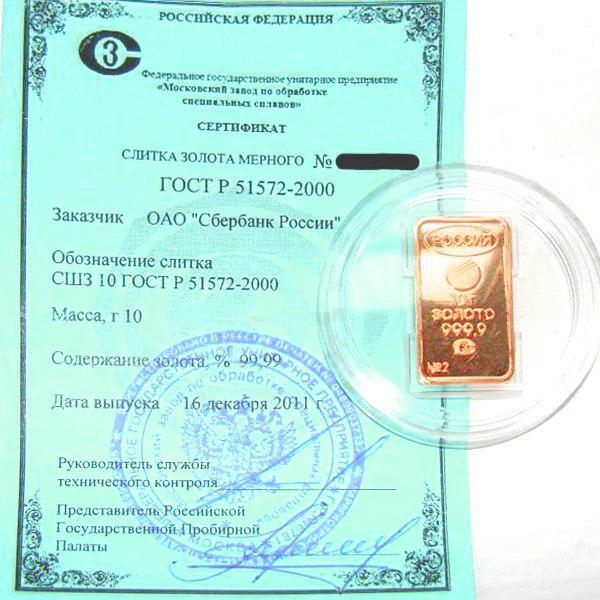
\includegraphics[width=1\linewidth]{p/vova.jpg}}
\end{center}
\end{minipage}
\hspace{5pt}
\begin{minipage}[h]{0.5\linewidth}
Для совершения операции с драгметаллами необходим \textbf{паспорт} или другой документ, удостоверяющий личность.

Каждый слиток сопровождается \textbf{\col{сертификатом качества}}, который является его своеобразным паспортом.
\end{minipage}

\vspace{5pt}
\begin{minipage}[h]{1\linewidth} 

Сделка оформляется \textbf{\col{актом приема-передачи}} и \textbf{\col{кассовыми документами}}.

Операции с драгметаллами в слитках облагаются \textbf{НДС} в размере \textbf{\col{20\%}}.
Однако, можно перевести слиток на \textbf{обезличенный металлический счет}.

\end{minipage}
		
		\end{frame}


		\begin{frame}
			\frametitle{Что по чем?}	
				По курсу на 30 ноября 180 000 евро = \textbf{13 374 000 руб}.
			  
			  \vspace{10pt}
			  \begin{center}
			  \textbf{\col{Стоимость слитка при обычной покупке}}
			  \vspace{5pt}
				\begin{tabular}{lc}
					Золото 1000 гр:  & 3 253 614	рублей \\
					Палладий 100 гр: &  327 391 рублей
				\end{tabular}

				\vspace{10pt}
			  \textbf{\col{Стоимость слитка при переводе на ОМС}}
			  \vspace{5pt}
				\begin{tabular}{lc}
					Золото 1000 гр:  & 2 755 000	рублей \\
					Палладий 100 гр: &  275 000 рублей
				\end{tabular}
    		\end{center}
		\end{frame}
		
		\begin{frame} \frametitle{Почему именно золото и палладий?}
		
		\begin{itemize}
		\item Золото много где используется и является оцень ценным материалом.
За последние три года стоимость золота выросла на \textbf{\col{14\%}} .

\vspace{10pt}
		\item Палладий очень сильно растет последние несколько лет.
За последние три года стоимость палладия выросла на \textbf{\col{114\%}}.
		\end{itemize}
		

		\end{frame}
		\begin{frame}
			\frametitle{Таблица за слиточек золота и палладия}
				\begin{minipage}[h]{0.5\linewidth}
				\begin{footnotesize}
				\begin{tabular}{ccc}
				\rowcolor{blue!30} Металл & Рост (\%) & Приб./Уб. \\
				\rowcolor{yellow!30}Золото & 14 & 45980\\
				\rowcolor{yellow!15} & 13 & 21410\\
				\rowcolor{yellow!30} & 12 & -3160\\
				\rowcolor{yellow!15} & 10 & -52300\\
				\rowcolor{gray!20}Палладий & 100 & 209000\\
				\rowcolor{gray!10} & 50 & 88000\\
				\rowcolor{gray!20} & 20 & 15400\\
				\rowcolor{gray!10} & 10 & -8800\\
				\end{tabular}
				\end{footnotesize}
				\end{minipage}
				\hspace{5pt}
				\begin{minipage}[h]{0.4\linewidth}
				\begin{center}
				{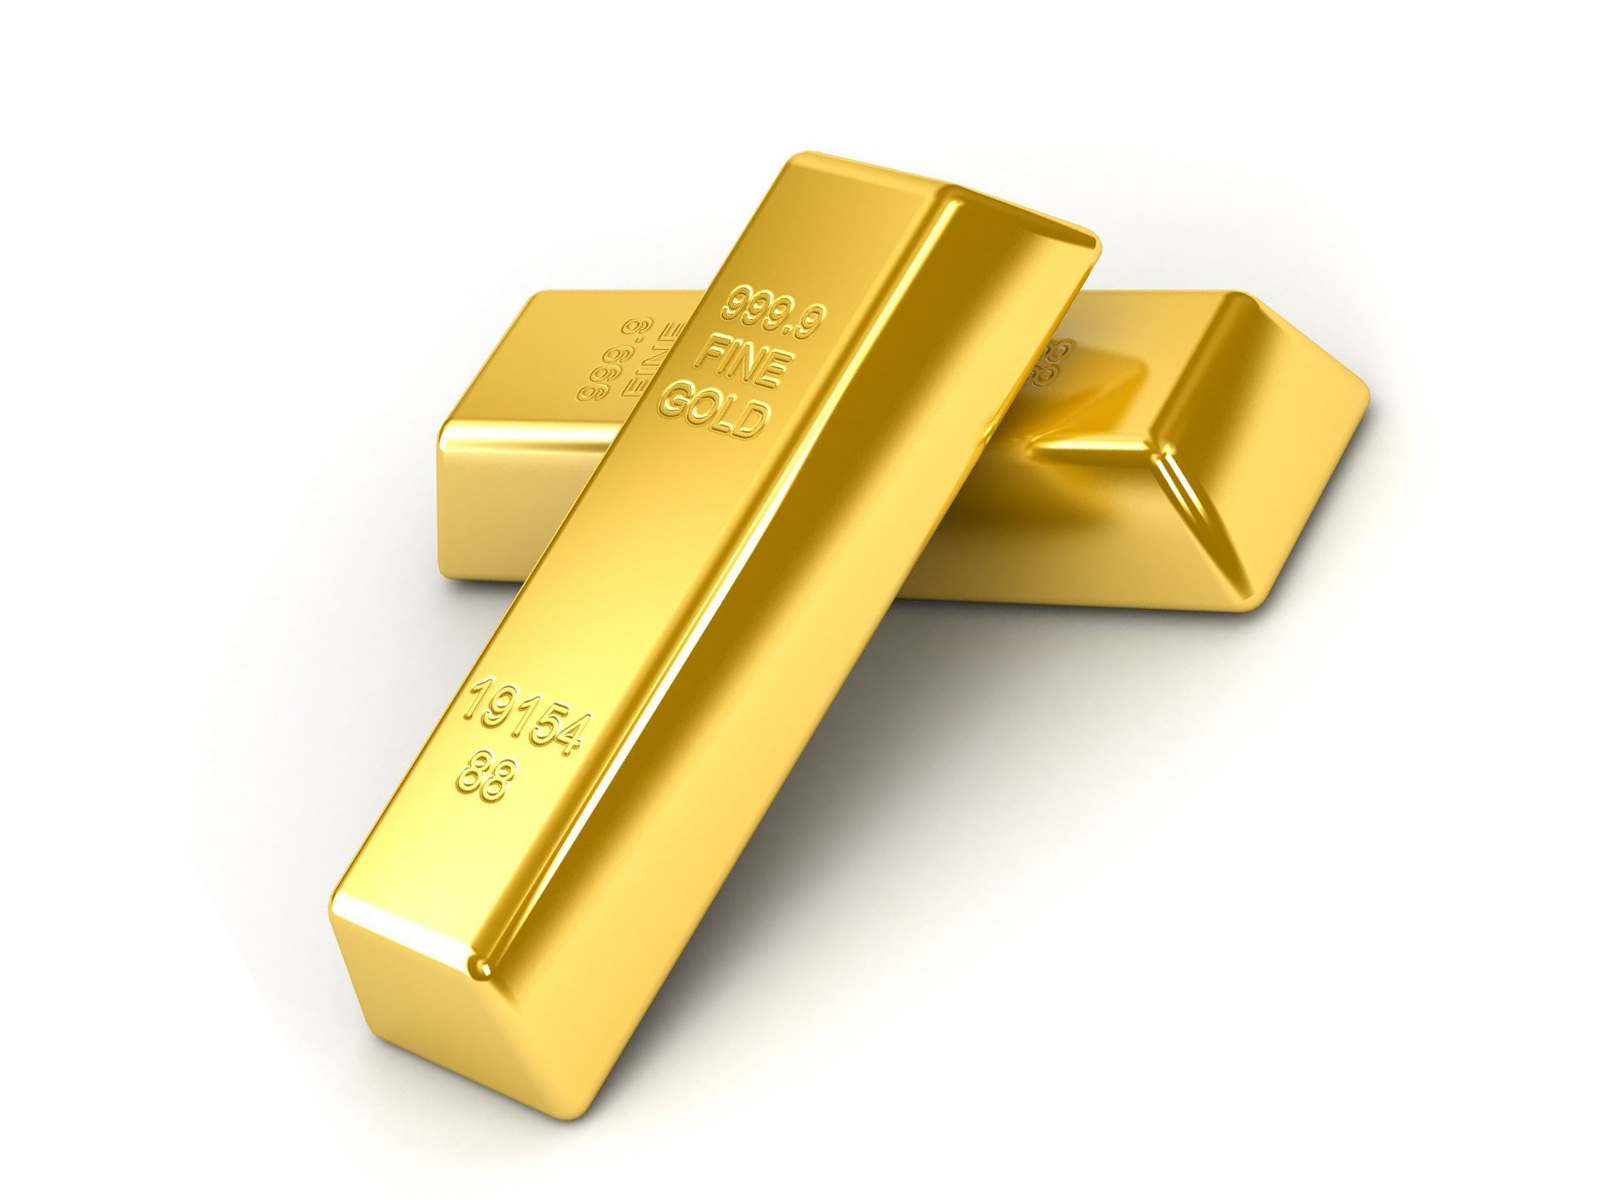
\includegraphics[width=1\linewidth]{p/metall.jpg}}
				
				{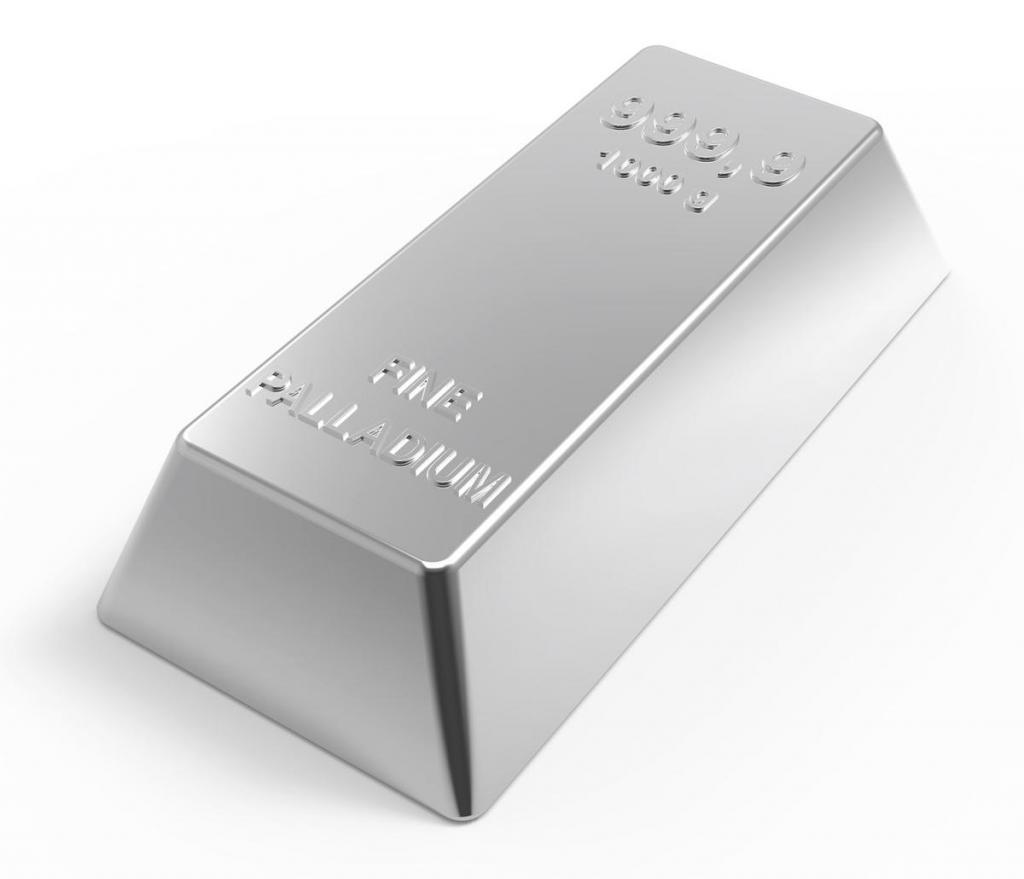
\includegraphics[width=1\linewidth]{p/2698408.jpg}}
				\end{center}
				\end{minipage}
						
						\end{frame}
				
				\section{Вклады в банки}
				\frame{
							\frametitle{Что важно?}
							\col{\textbf{Риски:}}
						\begin{itemize}
						\item Рост инфляции в стране
						\item Банк лишили лицензии
						\item ``Тетрадочные'' вклады
						\end{itemize}
						
						\col{\textbf{На что обратить внимание?}}
						\begin{itemize}
						\item Пополнение и снятие
						\item Выплата процентов
						\item Капитализаия
						\end{itemize}
				}
						
				\section{ОФЗ-н}
						\begin{frame}
							\frametitle{}
						
						
						\end{frame}
				
				\section{ИИС}
				
				
				\section{ПИФы}

\end{document}